\documentclass[12pt, a4paper,oneside, nocenter]{thesis}

%setting font to Arial and using UTF-8
\usepackage[utf8]{inputenc}
\usepackage[T1]{fontenc}
\usepackage[scaled]{uarial}
\renewcommand*\familydefault{\sfdefault} 

\usepackage{amsfonts}%checkmark

\usepackage{graphicx}%package for imges 
\usepackage{float}

\usepackage{tabularx}%table package
\usepackage{lastpage}%get page count
\usepackage{makecell}%multiline cell
\usepackage{multirow}%multirow
\usepackage{pdflscape}%for one page table

%centered columns P%
\usepackage{array}
%horizontal
\newcolumntype{P}[1]{>{\centering\arraybackslash}p{#1}}
%vertical
\newcolumntype{M}[1]{>{\centering\arraybackslash}m{#1}}

\usepackage{soul}
\usepackage[hyphens]{url}
\def\UrlBreaks{\do\/\do-}
\usepackage[hyphenbreaks]{breakurl}
\urlstyle{same}

\usepackage[normalem]{ulem}
\usepackage{xcolor}

\usepackage{etoolbox}
\usepackage{setspace}
\usepackage{wallpaper}
\usepackage{lipsum}
\usepackage{eurosym}
%\usepackage[none]{hyphenat}
%remove hyphenation
\tolerance=1
\emergencystretch=\maxdimen
\hyphenpenalty=10000
\hbadness=10000

\usepackage[document]{ragged2e}
\usepackage[font=small,labelfont=normal,figurename=Figure,labelsep=period]{caption} % Required for specifying captions to tables and figures
\captionsetup{justification=raggedright,singlelinecheck=false}

\usepackage[margin=1in,top=0.5in,includehead=true]{geometry}

\usepackage{cleveref}%setting figure referencing
\crefname{figure}{(Figure}{(Figure}
\creflabelformat{figure}{#2\textup{#1}#3)}
%%%%%%%%%%%%%%%%%%%%%%

\usepackage{titlesec}
\assignpagestyle{\chapter}{fancy}

% \ignore command for inline comments
\newcommand{\ignore}[2]{\hspace{0in}#2}

%Setting new line margins
\renewcommand{\baselinestretch}{1.5}

% package for todonotes
\usepackage[colorinlistoftodos,prependcaption,textsize=tiny]{todonotes}

\definecolor{olive}{rgb}{0.5, 0.5, 0.0}
\newcommand{\info}[2][1=]{\todo[linecolor=olive,backgroundcolor=olive!25,bordercolor=olive,#1]{#2}}
\newcommand{\improvement}[2][1=]{\todo[linecolor=Plum,backgroundcolor=Plum!25,bordercolor=Plum,#1]{#2}}


\usepackage{tocloft}%changing table of contents to dots
\renewcommand{\cftsecleader}{\cftdotfill{\cftdotsep}} % for sections
\renewcommand{\cftpartleader}{\cftdotfill{\cftdotsep}} % for parts
\renewcommand{\cftchapleader}{\cftdotfill{\cftdotsep}} % for chapters
\renewcommand\cftchapfont{\normalfont\fontsize{12}{12}\selectfont} % chapter font to 12\12
\renewcommand\cftchappagefont{\normalfont\fontsize{12}{12}\selectfont} %chapter page number font to 12\12

%headheight resetting error
\setlength{\headheight}{15pt}% ...at least 51.60004pt
%disabling identation for paragraphs
\setlength{\parindent}{0cm}
%increasing space before chapter
\setlength{\cftbeforechapskip}{2.5pt}

%style for chapters
\titleformat{\chapter}
[hang]
{\normalfont\fontsize{12}{12}\selectfont\bfseries}
{\thechapter}
{1em}{}

\titlespacing*{\chapter}{0pt}{-0.2cm}{0.3cm}
\titleformat*{\section}{\normalfont\fontsize{12}{12}\selectfont\bfseries}
\titleformat*{\subsection}{\normalfont\fontsize{12}{12}\selectfont\bfseries}
\titleformat*{\subsubsection}{\normalfont\fontsize{12}{12}\selectfont\bfseries}
\setlength{\parskip}{1em}

\usepackage{fancyhdr}%fancy headers/footers

\fancyhf{} % sets both header and footer to nothing
\fancyhead[C]{\thepage}

\fancypagestyle{plain}{%
\fancyhf{} % clear all header and footer fields
\fancyhead[C]{\thepage} %RO=right odd, RE=right even
\renewcommand{\headrulewidth}{0pt}
\renewcommand{\footrulewidth}{0pt}
}
%-- Stop figure counter resetting --%
\usepackage{chngcntr}
 
\counterwithout{figure}{chapter}
\counterwithout{table}{chapter}


\setcounter{section}{1}%start table of contents at 1

%-----------------------------------References------------------------------%
\usepackage[nottoc,notlot,notlof]{tocbibind}
\usepackage[comma]{natbib}
\bibliographystyle{xamk}
\renewcommand{\citep}[1]{(\citealp{#1}.)}
\newcommand{\citeyearxamk}[1]{(\citeyear{#1}.)}

%\bibliographystyle{dcu}

%move left
\setlength{\bibhang}{0pt}

%\renewcommand\harvardurl[1]{\RaggedRight\textbf{WWW %document:}
%\url{#1}}

\renewcommand{\bibname}{REFERENCES}
%-------------------------------------------------------------------------------%


% used in title page
\author{Aleksandar Ivanov}
\title{Educational AR/VR Systems for military projects}

\AtBeginDocument{% setting contents name to uppercase
  \let\mtcontentsname\contentsname
  \renewcommand\contentsname{\MakeUppercase\mtcontentsname}
}

\newcommand\blankpage{% used for adding an empty page
    \null
    \thispagestyle{empty}%
    \addtocounter{page}{-1}%
    \newpage}

\pagestyle{plain}
%%%%%%%%%%%%%%%%%%
%%%%%%%%%%%%%%%%%%
%%%%%%%%%%%%%%%%%%
%%%%%%%%%%%%%%%%%%
%%%%%%%%%%%%%%%%%% BEGINNING OF DOCUMENT
%%%%%%%%%%%%%%%%%%
%%%%%%%%%%%%%%%%%%
%%%%%%%%%%%%%%%%%%
\begin{document}

\pagenumbering{gobble}%removing page counter
% Set the right side of the footer to be the page number\fancyhead[R]{\thepage}

\makeatletter
\begin{titlepage}
	\begin{center}
	\ThisLRCornerWallPaper{1}{background.png}
		\vspace*{2cm}
		{\fontsize{16}{16}{\selectfont\@author}}\par
		\vspace{1cm}
		
		{ \setstretch{2.0}
			\fontsize{24}{24}{\selectfont\MakeUppercase{\@title}}
			
		}
		
		\vspace{1.5cm}
		{\setstretch{1.2}
			\fontsize{16}{16}\selectfont Bachelor's thesis \\ Information Technology
			
		}
        	
		\vspace{1.5cm}
        
		\fontsize{16}{16}\selectfont\the\year
        
		\vfill
		
\includegraphics{xamklogo}
		\vspace{0.8cm}
	\end{center}
\end{titlepage}
\makeatother
\pagenumbering{arabic}%starting page counter

%\blankpage
    \thispagestyle{empty}
    \noindent
    \begin{tabularx}{\linewidth}{|XXXX|}
      \hline
	   Author (authors) &  Degree &  & Time \\
	   Aleksandar Ivanov &  \multicolumn{2}{l}{Bachelor of Information Technology} & May 2019 \\
	   \hline
	   Thesis title & & & \\
	   \multicolumn{3}{|l}{Educational AR/VR Systems for Military Projects} & \pageref{LastPage} pages\\
	  \hline
	  Comissioned by & & & \\
	  \hline
	  Supervisor & & & \\
	  & & & \\
	  \hline
	  Abstract & & & \\
	  & & & \\
	  \hline
	  Keywords & & & \\
	  & & & \\
	  \hline
    \end{tabularx}

\newpage%TOC page
{\setstretch{1.2}
\tableofcontents
}

\newpage%first page with content

\newgeometry{top=1.25cm,left=4.0cm,right=2cm,bottom=1.25cm, head=14.5pt, includehead,includefoot,
  heightrounded,headsep=1cm}


%make title bold from outside so TOC stays the same
\chapter{\MakeUppercase{Introduction}}
Developments and improvements in computing technology have allowed for vastly improved immersion when consuming digital media. The most notable examples of such technologies are Augmented reality and Virtual reality. The immersion these technologies offer can be used to create educational systems that have more benefits than traditional digital education systems. \par
In this thesis project I will be comparing the differences between AR(Augmented reality) and VR(Virtual reality) in the context of educational software. Different implementations and physical devices will be compared and analyzed. A device and a technology will be chosen to create a prototype educational application for Observis Oy related to the company's Situational Awareness System(SAS).
\par 
The SAS product has a steep learning curve which raises the need for a more efficient educational tool. A training application that leverages newer technologies is the chosen approach to improve the training process. The primary goal of the training application is to provide a better view on the future prospects of using mixed reality for training. A secondary goal is to offer a training platform for better understanding of the ObSAS software to trainees. Furthermore finding other suitable AR/VR use cases for the current Observis projects can also be a positive by-product of the research.
\par
Advantages and disadvantages of AR/VR need to be considered over more traditional digital educational tools. The future prospects of these technologies are also of interest to the company. One reason for that is the growth of VR and AR popularity and market share over the recent years as the technology has improved \Cref{fig:ar-vr-consumer-spending}.
\begin{figure}[H]
	\centering
	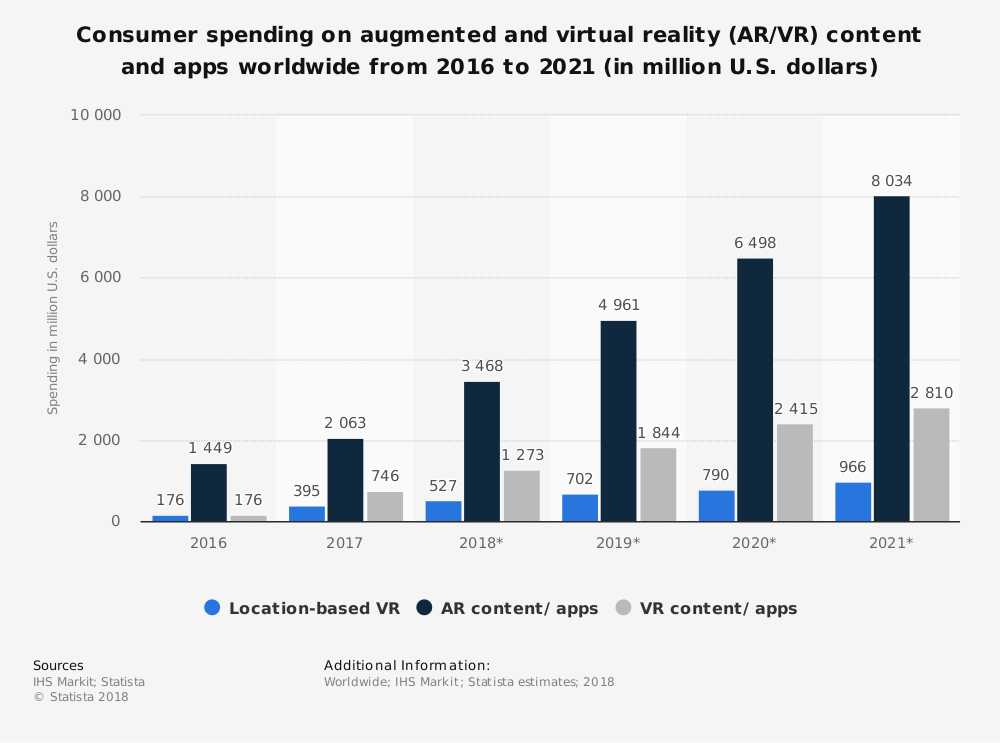
\includegraphics[height=210pt]{ar-vr-consumer-spending}
	\caption{Consumer spending on AR/VR worldwide 2016-2021 \citeyearpar{ar-vr-chart}}
	\label{fig:ar-vr-consumer-spending}
\end{figure}
Literature review is used as a research method for the first part of the thesis. The different literature in the fields of AR,VR and CBRN is reviewed and summarized. The second parth of the thesis is a case study of the practical implementation of a training application. The results will be analyzed by debating the success of the final product and its potential use.
\par
\chapter{\MakeUppercase{Augmented Reality and Virtual Reality}}
Augmented reality and Virtual reality are technologies that offer a different view and experience to the physical world. They leverage similar kinds of technology and both aim to provide an enhanced and enriched experience to the user. Both technologies are a part of the general area of mixed reality \Cref{fig:reality-virtuality}. However they have different goals and are essentially different in terms of user experience.

\begin{figure}[H]
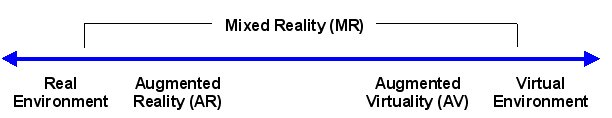
\includegraphics[width=\textwidth]{Virtuality_Continuum_2}
\caption{Reality-Virtuality Continuum (Paul Milgram et al. 2007)}
\label{fig:reality-virtuality}
\end{figure}

\section{Augmented Reality}%ref http://kjcomps.6te.net/upload/paper1%20.pdf
Augmented Reality(AR) can be described as the technology that bridges reality with virtual environments. Real life objects are transformed or replaced with virtual equivalents. Information can be added or removed to the real environment. Key aspects of AR are the ability to run in real time, be interactive, three dimensional and combine real with virtual information \Cref{fig:ar-application}. AR is most commonly used with the sense of sight, but it can potentially be used with other senses such as hearing, touch, smell, taste, temperature etc. AR can be considered as the next step in graphical user interfaces(GUI) evolution. \citep{prototyping-ar} Its current state is comparable to command line interfaces and 2d interfaces in the 1980's and 1990's. It is a vision of future computing and a field that is under research.
\begin{figure}[H]
	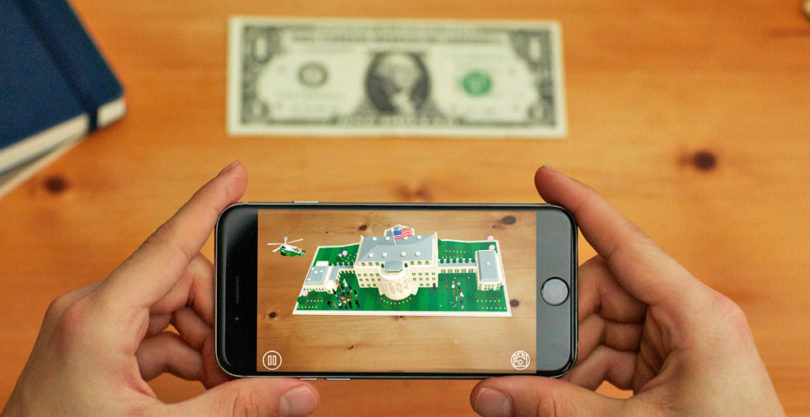
\includegraphics[width=\textwidth]{ar-application}
	\caption{Mobile Augmented Reality application \citeyearpar{ar-application-whitehouse}}
	\label{fig:ar-application}
\end{figure}
\par
Augmented Reality has higher technological requirements compared to VR which has lead to the slower maturity of AR. AR enabling technologies have been developed throughout the history of which the Optical see-through has become the most popular(Microsoft HoloLens, Google Glass, Intel's Vaunt). Optical see-through is achieved by using opaque displays on which virtual overlays can be rendered. The resolution of the real world is left intact as it passes through the screen. Benefits of this approach include power fail safety, which allows users to still see the real world even during a power outage, cheaper production costs of the used displays, no parallax effect that irritates the user's eyes. Disadvantages are the reduced visibility and brightness through the opaque lenses, limitation of the field-of-view, requirement of additional tracking sensors such as cameras, gyroscopes and accelerometers. Due to the lack of maturity of other AR enabling technologies only Optical see-through techniques will be considered throughout this work. \citep{vrjournal}
\subsection{AR for training and education}%ref https://files.eric.ed.gov/fulltext/ED510220.pdf
Augmented Reality provides new paths to conveying information. Learning experiences are more contextual by connecting and embedding information with the real world in real time. These approaches are already being utilised by Boeing. 
Mechanics in the company use AR goggles that aid repairs with embedded textual instructions, 
illustrate different steps of the repair and help users identify the required tools for a repair. 
Consequently training resources are reduced and transfer of information between workers is greatly 
improved. \citep{horizon-report}
\par
Learning through doing is another approach in which AR shines. Mistakes and errors made during the learning
experience have no real consequences. This provides for more authentic learning experiences which cannot be
achieved easily or cost effectively otherwise. \citep{augmented-reality}
\subsection{AR Challenges}
% As most developing technologies AR has many challenges that need to be overcome or improved. The requirements of the AR framework
% are directly related to those challenges.
An AR framework has basic requirements to accomplish a combination of the real and virtual world.
The four main requirements are sensing, tracking, interaction and displaying \Cref{fig:ar-framework}. Sensing refers to
capturing environment events and recognising markers or other objects of interest. Tracking handles updating the
viewing direction and position of the user relative to the real world. Tracking is an important component
of AR as even a slight tracking error can cause misalignment between the virtual and real world objects. \citep{ar-design} 
Registration refers to how the digital information is being delivered to the user. The registration can be achieved
through different methods for different senses: videos, audio, haptic feedback, scent, etc.
\begin{figure}[H]
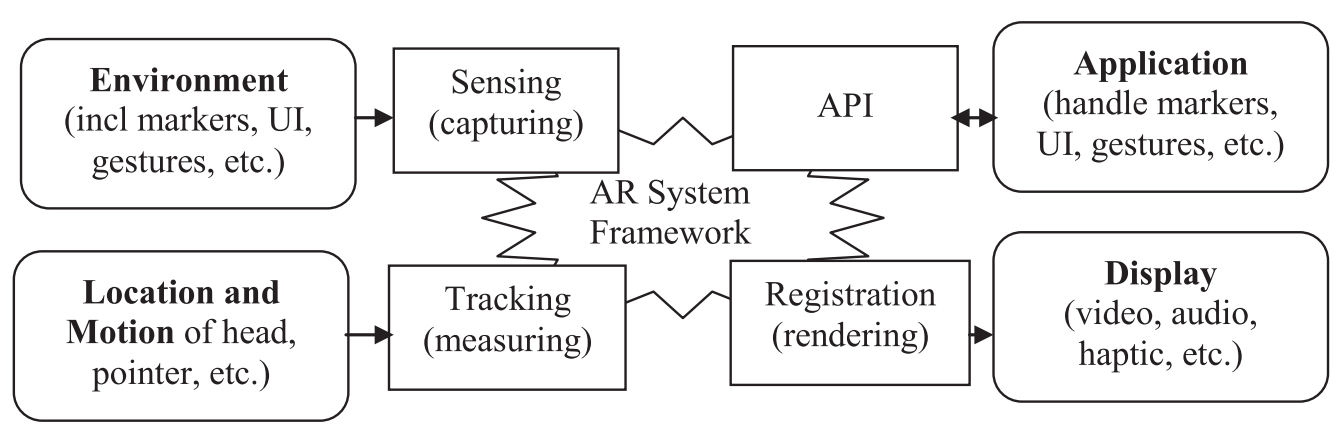
\includegraphics[width=\textwidth]{ar-framework}
\caption{Augmented Reality framework \citep{vrjournal}}
\label{fig:ar-framework}
\end{figure}
As most developing technologies AR has many challenges that need to be overcome before it can be widely adopted.
The challenges of AR arise from the framework requirements and they can be separated in five groups \Cref{fig:ar-challenges}.
\begin{figure}[H]
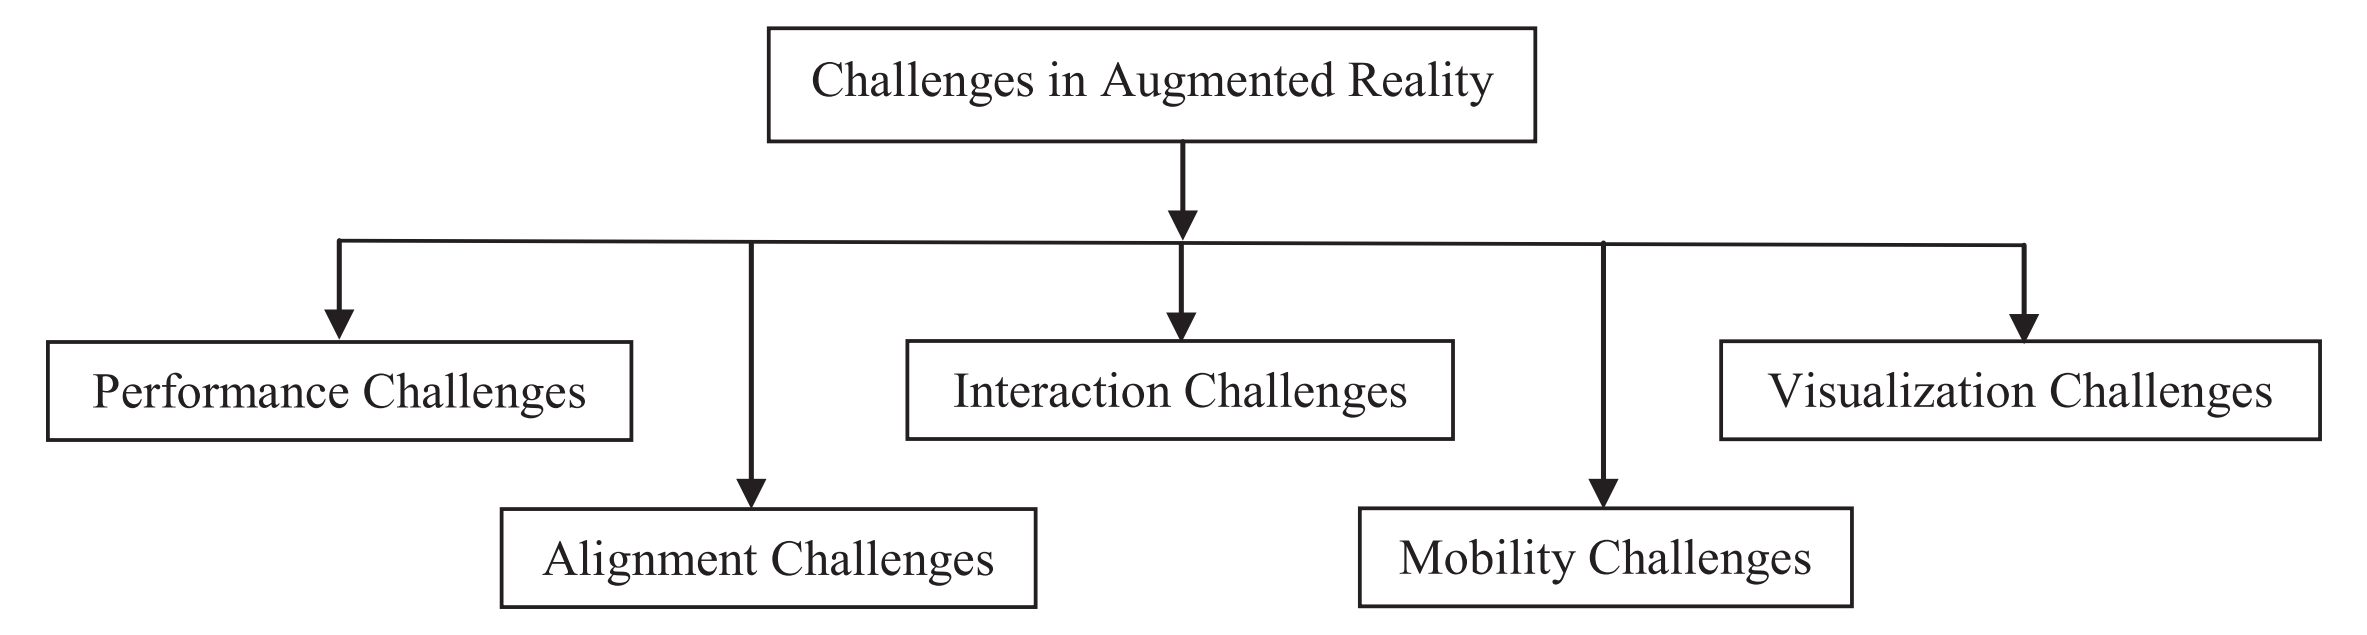
\includegraphics[width=\textwidth]{ar-challenges}
\caption{Augmented Reality challenges \citep{Acta-Graphica}}
\label{fig:ar-challenges}
\end{figure}
Performance challenges arise from the need of real time processing. AR tasks such as marker detection
and virtual object rendering are computationally intensive and this slows down performance.
Alignment challenges come from the complexity of tracking the users movement and registration of real
life objects. Any errors in those methods can cause misalignment between the rendered objects and
real view.\par
Interaction challenges are concerned with the interaction between users and virtual or real objects.
User interfaces need to be intuitive and unobstructive for the best experience. Mobility challenges refer
to the need of portability for AR systems.
\\
\section{Virtual Reality}
Virtual Reality(VR) in the broadest sense is the method or technology of substituting a physical environment with a virtually perceived environment. The Oxford dictionary gives a more detailed definition: 
''The computer-generated simulation of a three-dimensional image or environment that can be interacted with in a seemingly real or physical way by a person using special electronic equipment, such as a helmet with a screen inside or gloves fitted with sensors''.
This is typically achieved by using an HMD(Head mount display) with integrated motion tracking and a built-in or external rendering unit.
The requirements of VR are same to those of AR with the exclusion of environment sensing \Cref{fig:ar-framework}. The virtual environment
is entirely digitally constructed, thus eliminating the need for sensing as all environmental events are native to the system. It is achieved with a VR headset that has different views for each eye, accomplishing depth perception \Cref{fig:htc-vive-pro-headset}.
\begin{figure}[H]
	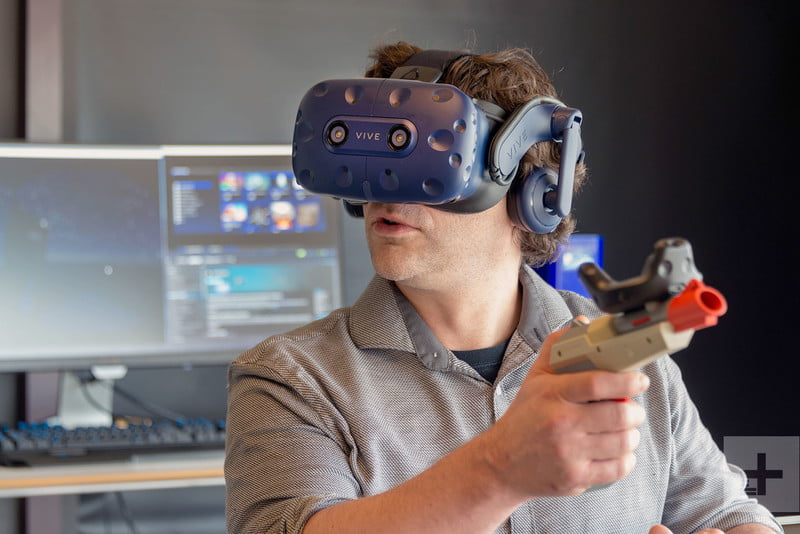
\includegraphics[width=\textwidth]{htc-vive-pro-headset}
	\caption{HTC VIVE Pro headset \citeyearpar{htc-vive-pro-review}}
	\label{fig:htc-vive-pro-headset}
\end{figure}
\par
Interaction with the environment isn't necessary for a VR experience, but it increases the possibilities and usability of a VR system.
Different approaches to user interaction offer various degrees of immersion and limitations. Motion tracked controllers, hand motion tracking gloves, pointer centered to the viewport, headset location tracking in 3D space and sekeletal motion tracking are common approaches.
\subsection{VR Challenges}
Virtual Reality challenges can be categorized in the same way as AR challenges \Cref{fig:ar-challenges}.
Performance is a very important factor in keeping the VR experience immersive for a prolonged period of time.
High resolution picture rendering at a high freamerate in real-time is taxing even for the highest end of current GPUs. 
Lower framerate or lower resolution picture can cause dizziness, eye tiredeness and overall dissatisfaction. Alignment challenges arise from the difficulty of tracking in real-time.
Users' view, location or controllers can become misaligned with the virtual environment, breaking the immersion and interactability.
Interaction challenges come from the current hardware limitations on interacting. Tactile feedback, hand interaction and free movement in the 3D space are all possible techniques individually, but combining them at the same time is not yet achievable.
\par %(Interrante et al., 2008; Mohler et al., 2010; Phillips et al., 2010).
Mobility challenges arise from the need of portability for VR platforms. Common solutions
rely on tethering to a machine that handles the rendering and power supply. However portable VR backpacks and headsets are starting to emerge a notable example of which is the HP VR backpack \citeyearpar{hp-vrbackpack}.
Visualization can be difficult due to the complexity of the physical world. Keeping proportions, lighting, textures, view depth, field of vision and other visiual perception aspects can be challenging.
\subsection{VR for education and training}
Virtual Reality has many prospects for use in education. Learning can be promoted by interacting with objects and the environment in a virtual world. 
Similarly self-paced exploration can improve the users' ability to understand a given topic.
%reference VR Collaborative learning
Learning through doing is even more prominent with VR than AR. Scenarios that are hard or impossible to create with traditional approaches can be executed in a virtual environment for the fraction of the cost.
Users that are physically apart can be in the same virtual environment.
Professors or specialists don't need to travel to remote locations to train people.
\section{Hybrid approaches}
\par
Hybrid approaches to VR and AR can be used to improve on some of the imposed drawbacks by the techologies. These approaches include using physical objects or combining different sensors.
Such a drawback for VR is the lack of tactile feedback or realistic hand interaction with the environment. This becomes a problem when training pilots as they get accustomed to the feel of the virtual environment and are unable to perform tasks as quickly in the real environment.
Feedback from the cockpit instruments is essential as well as the ability to use them with peripheral vision.
One solution to this problem has been developed by NLR(Royal Netherlands Aerospace Centre) with the use of a hybrid approach.
IR depth sensors and a camera feed are used to map the pilots hand in the virtual cockpit. Mockups of the flight instruments are 3D printed and are mapped to the virtual environment with tracking markers.
This allows for a much more natural feel of the flight instruments and offers better training results. \citep{nlr-vr}
\\
\section{Simulation training}
Simulation training is the process of using a controlled but competitive virtual environment to acquire real world skills. By implication the environment is an imitation of a real environment and the training is an imitiation of a real-life process. The process can also be recorded, analyzed and scored based on the results of the trainee. \citep{enterprise-simulation}
\par
Simulation training has been used for decades in the fields of  healthcare, military and aviation \citeyearpar{simulation-training-history} and several benefits have been observed. The simulated environment is safe and secure which allows trainees to practice and gain experience with the risk from mistakes being eliminated. Teamwork behaviours such as communication, collaboration, team leading can be improved in practice. Insight into the trainee's behaviour can also be obtained by recording and analyzing training sessions. \citep{medical-sim-training}
\par
In the military education field simulations are widely adopted. Strategy and tactics games have been used for officer training by the US Army forces. USA Command and General Staff College also uses a turn-based strategy game for their Crops-level operations course. Skill and Team Building has also has benefited from simulation training by using "first person shooter" games. Flight simulation is clearly one of the biggest beneficiary of simulation training according to an extensive study conducted by the US Navy. Higher scores were obtained by students who used the simulation product prior to the early flight training. \citep{games-sim-mil}
\par
With so many examples of good simulation training being effective and widely adopted it is possible to conclude that the SAS civil and military defense system can also benefit from such training.
\\
\chapter{\MakeUppercase{Project use case}}
Observis Oy is developing a product for situational awareness in different environments called ObSAS. This product is a software system running on multiple devices with multiple purposes. The product consists of several software packages with different purposes and providing different features. Depending on the project the required packages are selected and used. One main package is the low level software that communicates with various sensors and devices, such as chemical detectors, radiation sensors, biological detectors. Another package is the server software which summarizes the data and handles automatic actions. User software package allows users to interact
with all components of the system. The software packages can be integrated into varying environments and the final complexity of the product installation can also vary. Additionally required hardware and hardware installation support can be provided. Software support and maintenance can also be provided.
\par
The end use for the product is usually civil defence or shelter management. High reliability and availability are crucial requirements for the final product as human lives can be put in danger by improper operation of the software or misuse by the users. Training is necessary to ensure proper use of the software and 
other components of the situational awareness system. So far traditional training approaches have been used. Power Point slides including pictures of the software, textual description of individual components and narration from the training personnel.
\par
\section{Current training approach}
Current training is done on customers' premises in two parts - theoretical and practical. The theoretical part takes place in a classroom with teaching tools such as whiteboard and projector provided by the customer. A group of around 20 people is trained during the theoretical part with the use of powerpoint slides containing screen captures of the software. Additionally the software enabled in simulation mode is displayed and used in front of the trainees. Devices such as latops, external hard drives, cameras are not allowed during the training to avoid redistribution of confidential information.
\par
The second part of the training involves practical use of the system. One example project in which practical training was used is the Sassi case. In the Sassi Project case the training takes place inside a reconnaissance vehicle with a group of up to 4 people. Real life devices are used with the software. Test sources are used to trigger devices alarms and cable disconnecting is used to test failure states.
 Test sources or Simulants are compounds or biological samples that are used to verify proper operation of the detection devices. For chemical detection devices such simulants can be samples of acetone, ethanol, MSAL, acetic acid for Toxic Industrial Chemicals(TICs) and DMMP, DIMP for Chemical Warfare Agents(CWAs). The chemical simulants are provided at the air intake of the detection device and the time to alarm from exposure is observed. The time it takes for the device to clear out after the initial exposure is also monitored. These intervals can indicate if a device is operating correctly. The trainees are familiarised with these basic operations of the devices. More advanced operations such as creating reports, marking contamination areas, changing air intake directions are also practiced.
\par%switched to past perfect, not sure why, a bit inconsistent?
Feedback from the customer in the Sassi project has been positive, although there have been complaints from the trainees about the translation of the materials, but still overall positive feedback has been received. According to Jukka Härkönen(an employee from Observis who conducts the training) the trainees with better English language skills have managed to attain more knowledge from the training. Trainees who were familiar with a previous version of the software have had no problems adjusting to the differences in the new version of the product. Some trainees however have not been able to fully prepare for the use of the software and require further internal training conducted by the customer.
\section{Future goals}
Regardless of the good customer feedback there is room for improvement of the training. Streamlining the training can reduce the time required to create training materials and the amount of staff needed to conduct the training. Another future goal of the training is to be able to experience more lifelike situations and more complex scenarios resulting in better preparedness for critical situations. Misunderstanding caused by a language barrier is something that should be avoided in future training.
\par
Innovation in every aspect of the product is welcomed from the customers. The market has been stagnant and competing companies have been refusing to innovate due to the various risks involved with doing so. Observis is willing to take those risks to set itself apart. A survey and analysis of Virtual reality technologies interests the company.
\par
\section{Defining the application specifications and requirements}
A particularly sophisticated requirement of the system is the maintenance procedure. Measurement devices and sensors require periodic maintenance and inspection to remain in good operating condition. Negligence of these requirements can lead to faulty readings over time, device breakdown or even failure to recognise threats. The maintenance involves physical interaction with the measurement device that is guided by an instructional document. Software use is also required during the procedure to mark used parts and add additional notes. It is not possible to practice all maintenance procedures during training because of the time constraint. Consumables such as filters, batteries, tubings are often needed for the maintenance which can increase the cost of training. For the above-mentioned reasons implementing a training scenario that involves conducting a maintenance in a mixed reality environment would be of great benefit.
\par
One particular device that requires maintenance is Environics ChemProDM. The device is a Chemical Warfare Agents(CWA) and Toxic Industrial Chemicals(TIC) detector that is targeted for vehicle use \Cref{fig:chemprodm}. Typical installation includes 2 modules: ChemProDM detector and Remote Alarm Unit. A maintenance training scenario for this device is a great candidate for a mixed reality application. Initial installation and testing are also interesting use cases that can benefit from a training application.
\begin{figure}[H]
	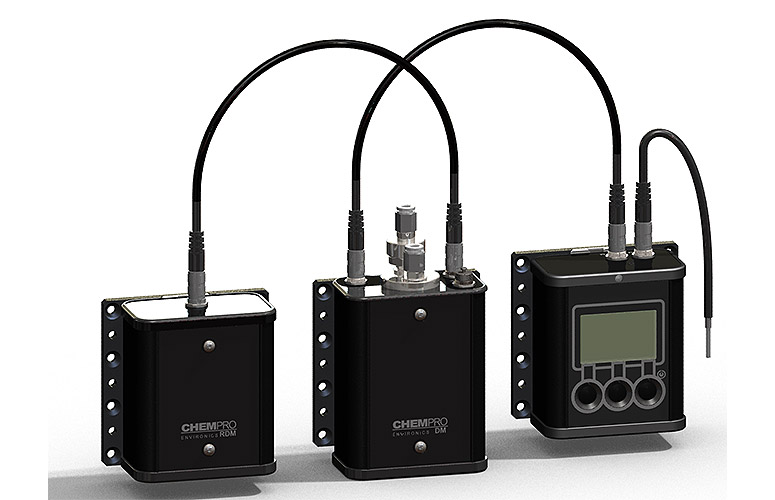
\includegraphics[width=\textwidth]{chemprodm}
	\caption{ChemProDM and modules \citeyearpar{environics-chemprodm}}
	\label{fig:chemprodm}
\end{figure}
\par
Other devices included in ObSAS are Thermo SVG2 radiation sensor, Meteo IRDAM MAWS 5060 weather sensor, Infinicon Hapsite ER chemical analyzer. Basic knowledge of those devices is a great benefit when using the system, however it is not required of the users. The user can be familiarized with the devices during training. The knowledge attained can be helpful if on field repairs are required.
\par
\subsection{CBRNe defense}
CBRNe is an acronym for Chemical, Biological, Radiological, Nuclear and Explosives. CBRNe defense is the field of detecting, reducing the impact of or avoiding the threats of CBRNe agents. In recent years the threat of CBRNe attacks has increased due to technological development and increased willingness of terrorists to obtain and use such agents. \citep{crowd-behavior}
\par
A motivation for CBRNe defense is the amount of casualties taken by CBRNe threats all around the world all the time. Such incidents are covered bi-monthly in the CBRNeWORLD magazine and their numbers are not decreasing \citeyearpar{cbrne-world}. The industry in this field aims to provide solutions that prevent or reduce the impact of CBRN incidents and attacks. Market share of the field has been growing steadily and the forecast is of continuous growth for the future years to come according to Visiongain's market report \citeyearpar{cbrn-market-share}.
\par
ObSAS provides possibilites for early detection and prevention of CBRN attacks. Gathering as much information possible about the attack can help with planning impact reduction and prevention strategies. ObSAS allows for the gathering and analysis of such data: chemical threat identification, air spectrum analysis, radiation measurement, geographical location and meteorological conditions. A vehicle with an ObSAS installation can safely cover and inspect a large area. Communication channels can be used to share and collect data from various CBRN sources. A more clear picture of threats can be established that way.\par
The CBRN field also encompasses considerations such as decontaminating equipment and clothes, medicine administration, using protective equipment and detection devices require training and practice. Databases providing instructions on what actions to take depending on the threat are often available in CBRN software. The use of such databases also benefits from prior training.
\section{Comparing VR and AR in the project context}
AR and VR differ not only in hardware but also in software development kits. It is rarely the case that an application written for one of the platforms can be seamlessly ported to the other. Therefore the two technologies need to be compared in regards to the current project. To keep the scope of this thesis narrow a single technology will be used to implement a training application.
\par
AR hardware such as goggles, glasses and headsets are generally very portable and self-contained. This makes it easy to transport the required hardware during training or installation tirps. The initial setup of the training environment could be more tedious with AR. If real life devices need to be tracked, markers have to be placed and calibrated. As seen from the specification sheet on the Microsoft store \citeyearpar{hololens-specs}, the HoloLens have narrow field of view, smaller color space, low luminosity and lower computing power compared to VR headsets. This can result is reduced immersion and engagement with the virtual environment. Another downside is the inability to emulate real life scenarios such as being inside a moving vehicle or simulating an environment that is completely different from the one the user is in. For example it is impossible to simulate night missions if the user is in a brightly lit room. For these reasons AR is restricted by the environment it is being experienced in.
\par
The easability of use of AR headsets is one important benefit. While VR headsets require a tether cable, external computer and even base stations in some cases, AR headsets can be used as they are, independently. 3D modelling isn't as big of a requirement compared to VR as it is enough to create models only of the objects the user interacts with, not the full environment the user is in. This can reduce development time significantly.
\par
VR shines in implementing a completely independant environment. The only limit to what can be recreated is imposed by the hardware performance and development time and skills. VR allows for spectating and recording users' interaction with the environment. This can be used to analyze their experience and improve the software further. Giving suggestions and guiding during the training is also possible. A multi-user environment is also possible and trainees and teachers can be in the same environment even if they're physically far apart.
\par
Price difference is very small between VR and AR if the most advanced frameworks are being considered. An AR headset with the development pack such as Microsoft HoloLens is priced at 3000\$ on the Microsoft store \citeyearpar{hololens-price}. And a VR headset such as HTC Vive Pro is priced at 1500\euro\ on the official VIVE store \citeyearpar{htc-vive-pro} with VR capable laptops priced starting from 1500\euro. Similarly prices of development kit licenses are not far apart either. This makes the decision between the two based entirely on the features they provide, driven by the requirements of the use case they're aimed for.
\par
\section{Selection of mixed reality framework}
The main benefit of AR over VR in this project is the portability and ease of use it offers. In terms of what training can be implemented VR offers a lot more possibilities. Battery limitations are also reduced or avoided which enables long training sessions. Good multiplayer support and additional peripherals(such as gloves and controllers) are in favor of VR too. The portability of AR is not a crucial feature for this project and the usability it offers over VR are not sufficient enough to place AR as a more suitable platform in this project. A conclusion to this chapter is that a VR framework is a more suitable choice in the context of creating a training application for the ObSAS system.
\par
\chapter{\MakeUppercase{Project definition}}
This chapter will describe the virtual application in more detail and outline the different technologies used in the implementation. Concepts such as 3D computer graphics, 3D modelling, game engine and tracking will be defined. Source code used in the development of the application will be provided and explained.
\par
\section{Researching VR hardware and software}
The most notable VR headsets available on the market are Occulus Rift and the successor to HTC VIVE, the HTC VIVE Pro. Widest software and peripheral support is offered to these headsets, so other options would not be considered. The main difference between the two is that HTC VIVE Pro has higher screen resolution and pixel density \Cref{fig:comparison-table}. Occulust Rift has lighter controllers, but requires at least 3 or even 4 sensors in some cases for decent room tracking. In contrast HTC VIVE Pro offers a wider tracking area with just 2 tracking sensors as pointed out by WindowsCentral VIVE Pro vs Occulus Rift article \citeyearpar{vive-vs-rift}. Both options provide the required features, but HTC VIVE Pro is more suitable and offers more because of the better graphics. 
\begin{figure}[H]
	\begin{tabular}{|l|l|l|}
	\hline
	\textbf{Category}   & \textbf{HTC VIVE Pro}                                               & \textbf{Occulus Rift}                                                \\ \hline 
	\textbf{Display}    & Dual Amoled 3.5                                                   & Dual Amoled 3.54"                                                    \\ \hline
	\textbf{Resolution} & 1440x1600(2880x 1600)                                               & 1080x1200(2160x1200)                                                 \\ \hline
	\textbf{PPI}        & 615                                                                 & 461                                                                  \\ \hline
	\textbf{FOV}        & 110 degrees                                                         & 110 degrees                                                          \\ \hline
	\textbf{FOV}        & 90Hz                                                                & 90Hz                                                                 \\ \hline
	\textbf{Connection} & \begin{tabular}[c]{@{}l@{}}USB-C 3.0\\ DisplayPort 1.2\end{tabular} & \begin{tabular}[c]{@{}l@{}}HDMI\\ USB-A 2.0\\ USB-A 3.0\end{tabular} \\ \hline
	\end{tabular}
	\caption{HTC VIVE Pro vs Occulus Rift specs}
	\label{fig:comparison-table}
\end{figure}
VR hand and finger tracking is a great addition to the immersion of the VR experience. More intuitive interaction with the virtual environment is possible. Many gloves are available as prototypes on the market. Some feature resistive finger feedback and texture and shape simulation like the VRGluv \citeyearpar{vrgluv}. A large portion of such gloves are in the prototyping stage and can only be preordered. The Noitom hi5 gloves however are available as a purchasable product, even though they're missing the aforementioned features.
\par
These gloves achieve full finger tracking by using 9 inertial measurement units on each glove. The VR headset controllers are strapped on the gloves to provide absolute tracking \Cref{fig:vr-glove}. Vibration feedback is also supported by the hardware and software API as documented by Noitom on their product website \citeyearpar{hi5-vr-glove}.
\begin{figure}[H]
	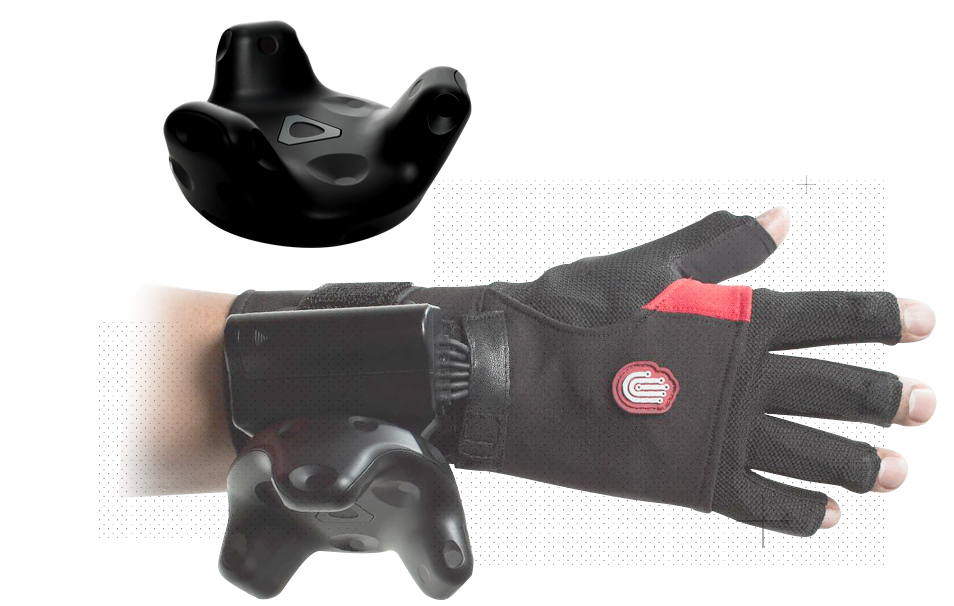
\includegraphics[height=210pt]{vr-glove2}
	\caption{Noitom HI5 VR glove \citeyearpar{hi5-vr-glove}}
	\label{fig:vr-glove}
\end{figure}
\par
The Noitom hi5 gloves are compatible with HTC VIVE Pro and offer SDKs for the most popular game engines (Unreal Engine and Unity). These gloves will be used in the project to achieve better immersion and quality of training.
\section{Game engines}
A game engine is a software framework aimed at simplifying and streamlining the production of games. At the core it provides a 3D or 2D rendering engine, generic physics engine, sound, animation and other features that assist game creation but do not directly specify the game's behavior. If used successfully a game engine can produce a higher quality game with less resources and in less time. An engine isn't required to build applications as all the features can be implemented from the ground up without the need for reusability or modularity, but that takes significantly more resources than using already existing tools. \citep{game-engines}
\par
Despite having the name game engine, such engines have many other applications besides making games. They can be used for pretty much any graphical application. Simulation applications, training applications, VR and AR applications of any kind, presentations, cinematography can all benefit from using a game engine. Using a game engine is suitable for this project because of the time constraint and limited resources available. 
\par
One popular game engine is Unreal Engine, created by Epic Games Inc. It is widely adopted and it offers a large selection of plugins, addons, libraries and assets that aid development. Unreal Engine supports various VR and AR platforms including HTC VIVE Pro and Hi5 vr gloves. This engine will be used to develop the training application.
\section{Application Objectives}
The application objectives can be defined as a set of actions that the user needs to complete in a certain order. Using objectives helps quantifying the training progress and give guidance to the user at the same time. Having structured objectives also helps motivate users to continue interacting with the software. \citep{goal-oriented-games}
\par
Defining the application objectives also helps the development process. In the context of this 3D application the required assets can be inferred from the application objectives. These assets include 3D models the user interacts with, sound effects, written instructions, 2D graphics, background environment models. Gathering a list of these assets and their description is necessary for outsourcing the 3D modelling work or sound effect composition. Such topics are out of the scope of this thesis, therefore the production process of the used assets will not be covered.
\par
The training will take place inside a virtual environment. This virtual environment consists of the interior of a vehicle, all detection devices, computational devices, power distrubition and sampling system. The first objective is to explore the vehicle and get acquainted with the environment. The second objective is to check whether all connectors are plugged at the correct places and inspect all cables for visual signs of wear. The third objective is to power up the entire system and wait for baseline acquirement of all detection devices. Once that is complete the next objective is to begin chemical detection tests with simulants. If the simulant causes a chemical alarm the user will also be required to acknowledge that alarm and print a report.
\par
The next objective is to test radio-nuclear detection by using a sample of radioactive rock ore. Again if an alarm is prompted the same actions need to be repeated. Afterwards biological detection is tested with simulants. The last objective is to assure that the system has reached baseline operation again and then shut it down.
\par
With the list of objectives defined in the table below it is possible to create a list of the required 3D models \Cref{fig:objectives-table}. This list can be used to request modelling work, which will be done internally at Observis Oy. Obtaining 3D models of the detection devices proved to be difficult as companies are not willing to provide these without any ongoing projects related to the devices.
\par
All the objectives take place in a relatively small area which means they can be a part of a single Level. Unreal Engine Levels are explained in the next section.
\begin{figure}[H]
	\centering
	\begin{tabular}{@{} |M{0.45cm}|p{2.5cm}|p{6.5cm}|M{2.4cm} |@{}}
	\hline
	\textbf{\#} & \textbf{Description}        & \textbf{Models}                                            & \textbf{Compulsory} \\ \hline
	1           & Explore the vehicle         & Vehicle                                                    & \checkmark          \\ \hline
	2           & Check connections           & Wires, Plugs, Sockets, Power/Junction box                  & \checkmark          \\ \hline
	3           & Power up the system         & Power switch, Indication lights, Display and Computer      & \checkmark          \\ \hline
	4           & Chemical simulant testing   & Chemical simulant, Chemical detector, Air sampling box     & \checkmark          \\ \hline
	5           & Chemical Alarm              & Keyboard, Mouse, Laptop/Computer                           &                     \\ \hline
	6           & Radiological testing        & Radiological detector, radioactive sample                  & \checkmark          \\ \hline
	7           & Radiological Alarm          & Keyboard, Mouse, Laptop/Computer                           &                     \\ \hline
	8           & Biological simulant testing & Biological detector, Biological simulant, Air sampling box & \checkmark           \\ \hline
	9           & Biological Alarm            & Keyboard, Mouse, Laptop/Computer                           &                     \\ \hline
	10          & System shutdown             & Power switch, Indication lights, Display and Computer      & \checkmark           \\ \hline
	\end{tabular}
	\caption{List of Objectives and required 3D models}
	\label{fig:objectives-table}
\end{figure}
\par
\section{Unreal Engine Level}
Levels are defined in Unreal Engine's documentation as a collection of Static Meshes, Volumes, Blueprints and other entities that the user sees and interacts with \citeyearpar{ue-levels}. They are helpful to organize a project into different virtual locations or chronologically. Levels are treated similarly to other assets in UE. They can be created, loaded and modified from the Content Browser.
\par
The full training takes place inside a virtual vehicle, which can be accomplished by using a single level. UE4 comes with starter content when creating a new project. One level that comes with the VR project template is the MotionControllerMap \Cref{fig:level-ue4-editor}. This level features a VRPawn object which is responsible for the majority of functionalities related to the user. It handles tracking of the Head Mounted Display and syncing camera to it, input from controllers, mapping the controllers' location to static meshes, player positioning in the environment and others.
\begin{figure}[H]
	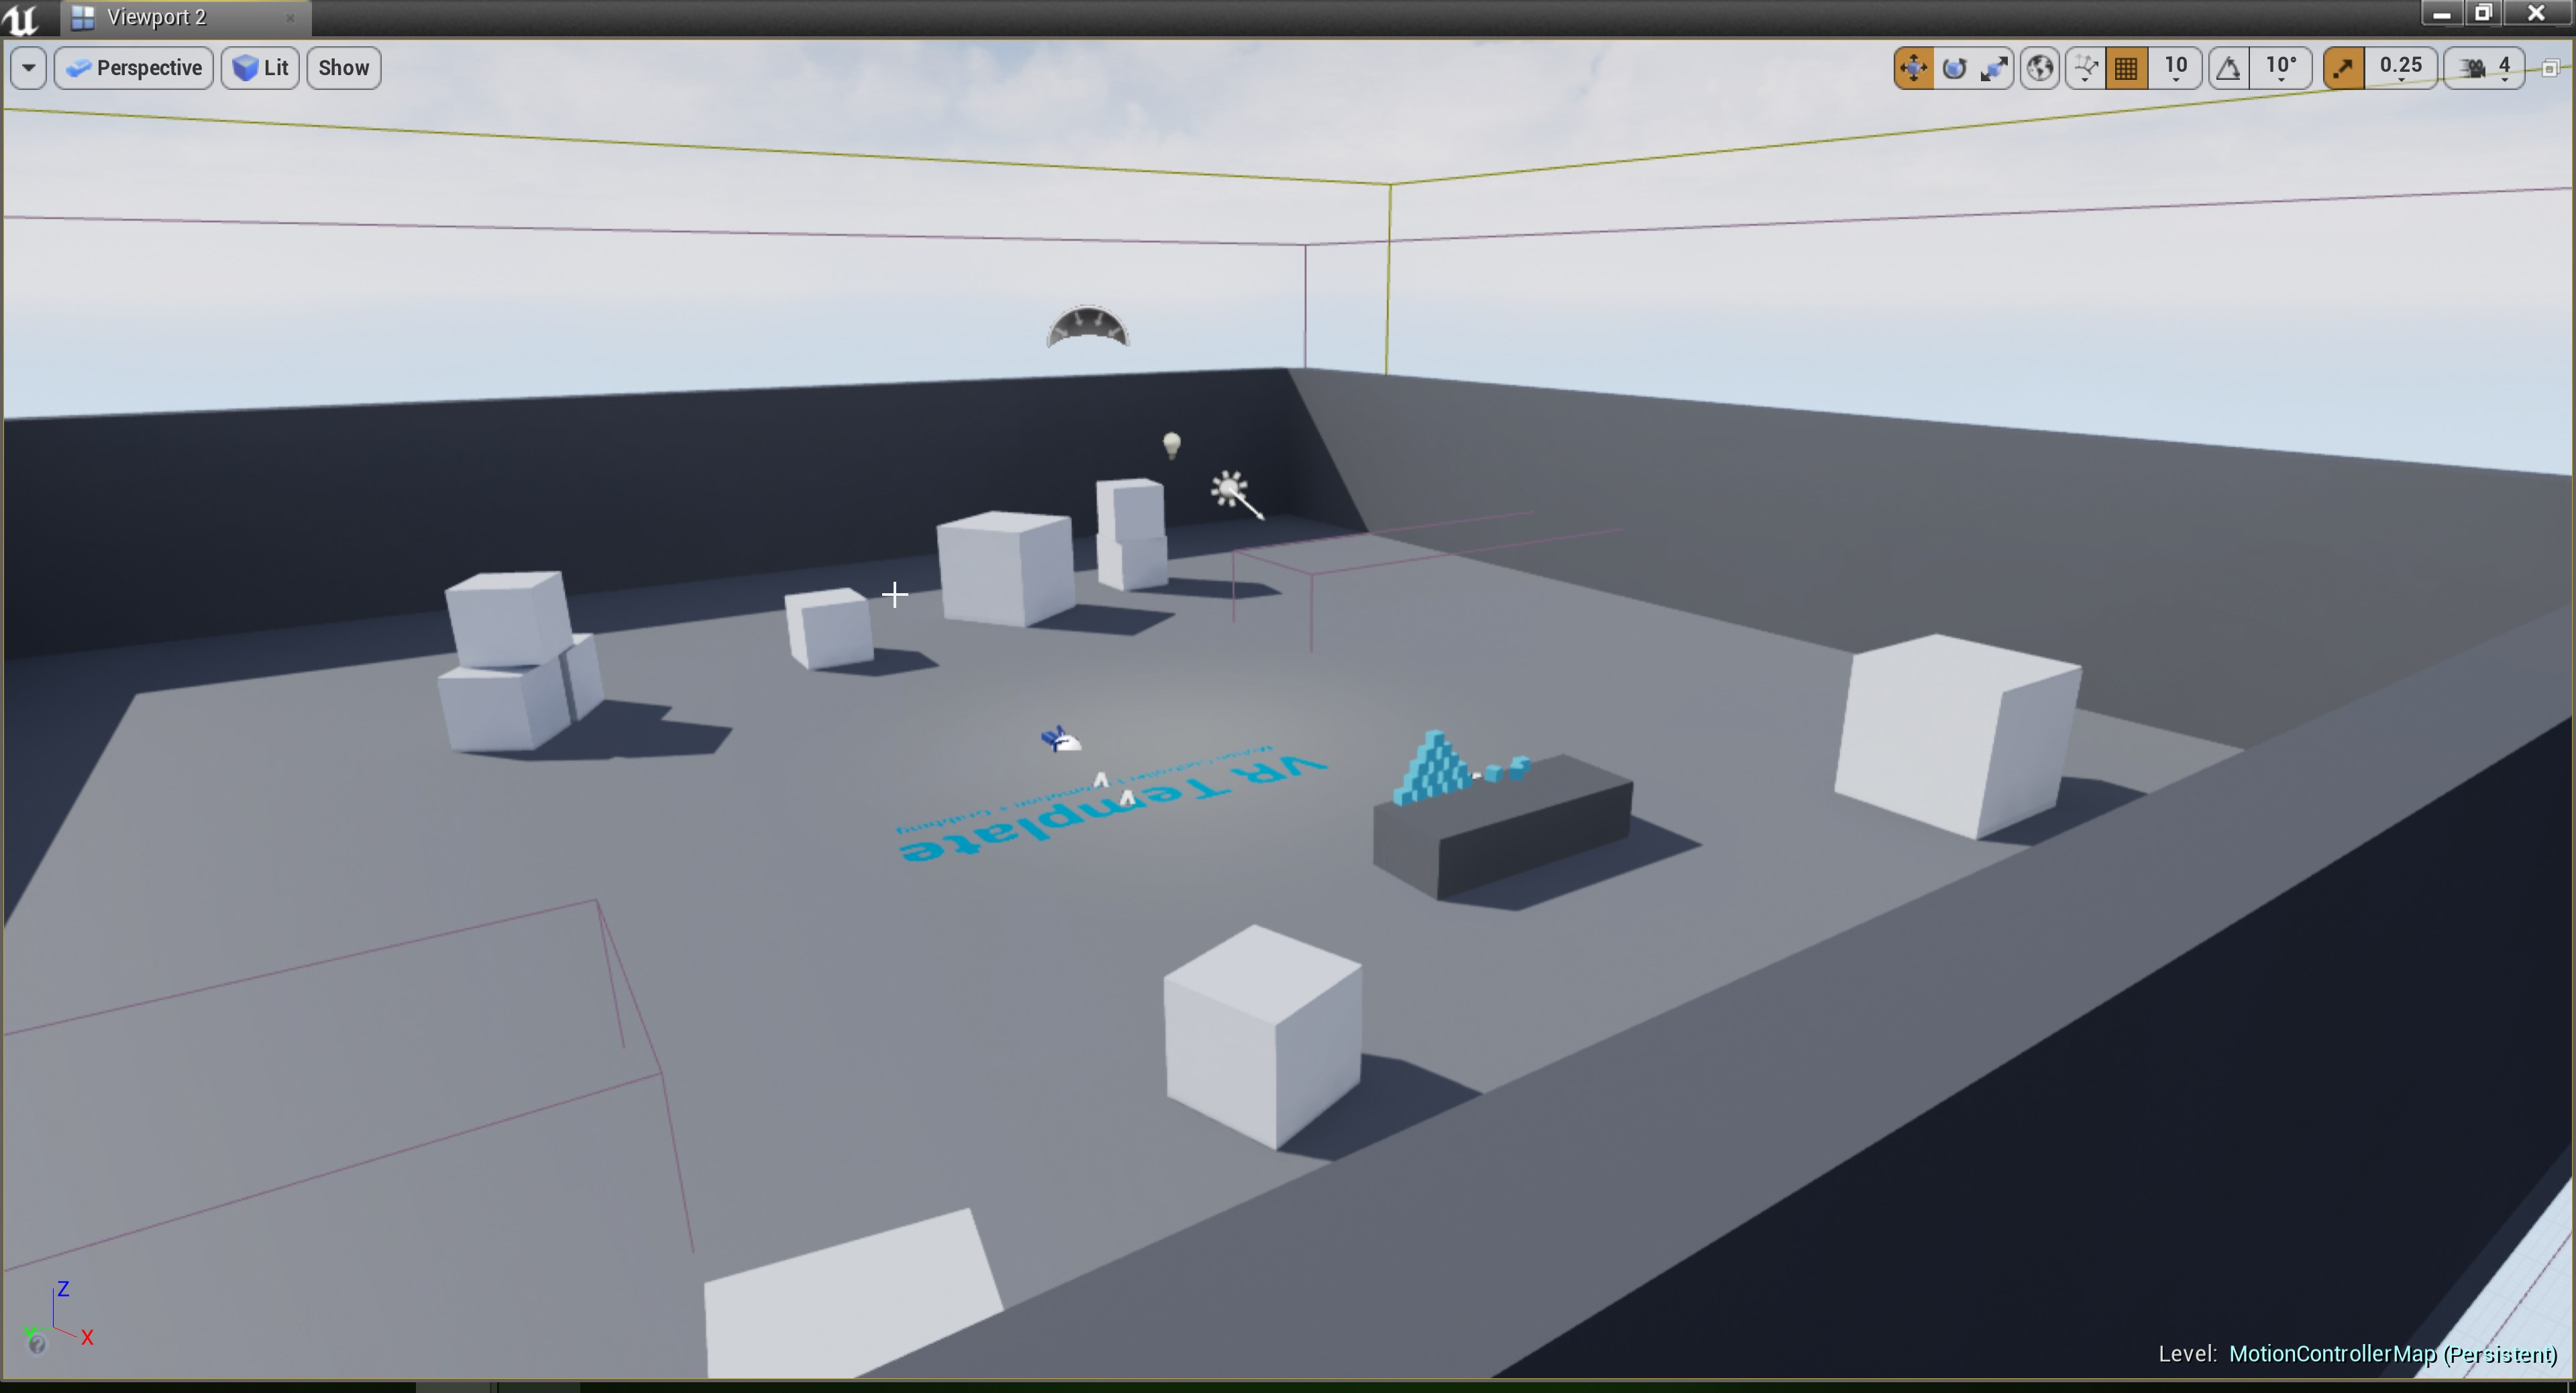
\includegraphics[width=\textwidth]{level-ue4-editor}
	\caption{UE4 MotionControllerMap Level Viewport}
	\label{fig:level-ue4-editor}
\end{figure}
Other objects in this level are the different light entities which include ambient light, point light, sky light and light interaction and postprocessing. This level also comes with several meshes, some of which have simulated physics interaction. And the last type of components in this level are the NavMeshBoundsVolume and NavModifierVolume entities which define what areas in the level the user can walk on.
\par
This starter content level provides all the basic functionalities needed for this project. It can be used as a starting point for the implementation and further extended and modified to contain the full training. In the future more levels can be added for different locations and scenarios.
\subsection{Actors}
Actors are generic Classes in UE that support 3D transformations such as transformation, rotation and scaling. These actors can be created(spawned) and destroyed dynamically while the application is running. They can also be updated dynamically by "ticking", which means that they can be updated with every rendered frame(tick). Another main function of Actors is replication and controlling behaviour of objects in network play(multiplayer). Actors hold different types of objects which are called Components, in a sense Actors are containers for Components. The main types of Components Actors can hold are UActorComponent, USceneComponent, UPrimitiveComponent. UActorComponents have conceptual functionality, they don't exist anywhere in the world. They can be used for example to implement AI functionality, handle user input, saving/loading game progress. USceneComponents are placed in the world and have a location, scale and rotation parameters. UPrimitiveComponents have graphical presentation from a static mesh, particle system, 2D graphics or other primitive assets. Physics, collision and overlap settings are available for these components.  
\par
Some examples of actors in this project are StaticMeshActors of the different detection devices, CameraActor responsible for what the player sees, PlayerStartActor that defines the player starting point. Actors are also hierarchical with one Root Actor having nested Actors on several levels. Controlling the actors can be done with gameplay code written in C++ or with blueprints. \citeyearxamk{ue-actors}
\subsection{Blueprints}
Blueprint is a visual scripting tool in Unreal Engine that offers the full range of development tools and concepts generally available only to programmers. A node-based visual interface is used in which different Events, Nodes, Functions and Variables are connected with Wires \Cref{fig:ue-blueprint-tool}. These connections can define complex gameplay logic by combining and chaning multiple simple operations and creating conditional logic. Objects created with this visual tool are referred to as Blueprints. \citeyearxamk{ue-blueprints}
\begin{figure}[H]
	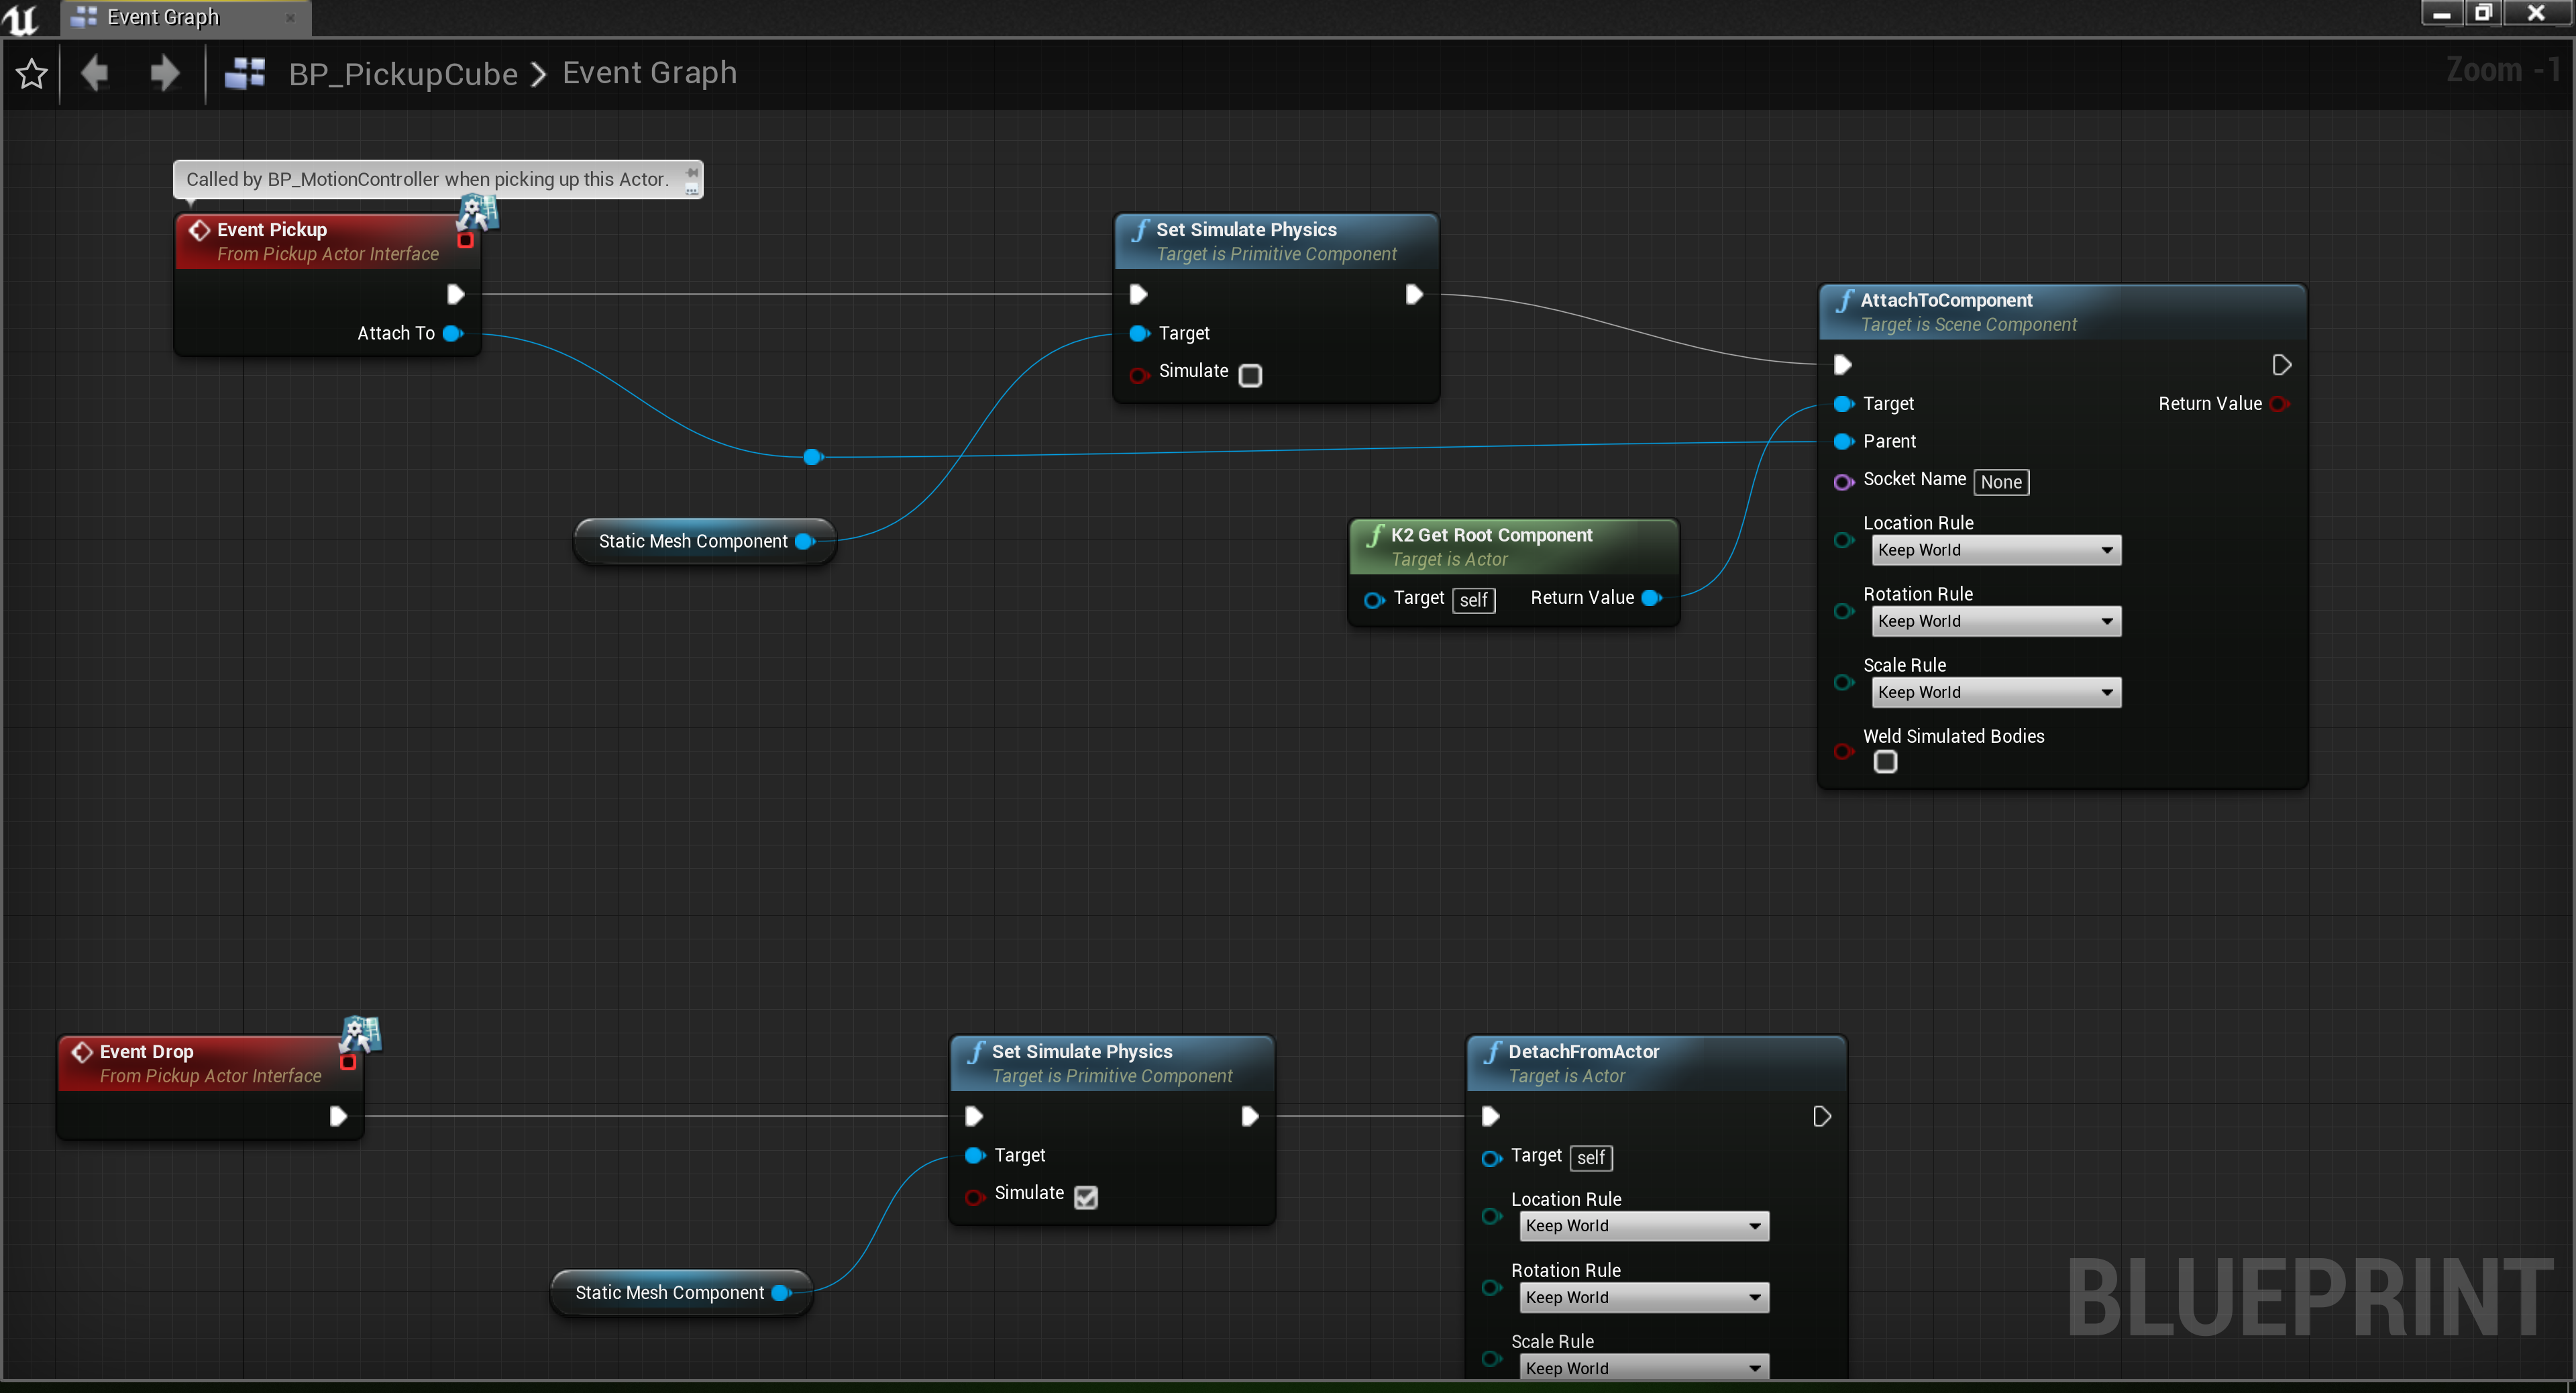
\includegraphics[width=\textwidth]{ue-blueprint-tool}
	\caption{UE4 Blueprint Visual Editor}
	\label{fig:ue-blueprint-tool}
\end{figure}
\par
Blueprints are defined as object-oriented(OO) classes or objects in the engine which is a well known and used programming paradigm. Internally Blueprints are translated to C++ by a VM which comes with a performance penalty \citeyearpar{ue-nativizing-blueprints}. An alternative to Blueprints is using C++ to define the game logic, however in this project Blueprints are favored due to their ability to visually display logic better than code. There are also more examples and snippets online available for blueprints.
\par
Two common types of Blueprints are Level Blueprints and Blueprint Classes. Every level has a Level Blueprint which can manage things like level streaming, objective tracking(checkpoints), interacting with other blueprints in the level. Blueprint Classes on the other hand are used to create interactive assets such as doors, buttons, levers, destructible objects. Main benefit of these blueprints is their reusability. They can be placed in any level and their behavior will remain the same. Also modifying the base blueprint will update all instances of it in the level.
\par
\chapter{\MakeUppercase{Project implementation}}
This chapter covers the practical implementation of the project application. Level layout and design is created and explained. Blueprints defining the game logic are also created and explained. Other various steps of the implementation process are listed and discussed.
\section{Level design}
Level design begins with the layout and orientation of the different meshes. The visual appearance of the level is made more realistic by using different textures, materials and lighting. A vehicle 3D model is used as the center point for the level and also for the player starting point.
\par
The player starting point is placed in the interior of a conversion van \Cref{fig:vehicle-interior}. If the starting point Actor is colliding with objects in the scene an icon "BADsize" will appear. This means that the starting point is invalid and the engine will try to find the nearest valid starting point. During the development process the camera location in the editor can be used as a strating point which speeds up testing. \citeyearpar{ue-playerstart}
\begin{figure}[H]
	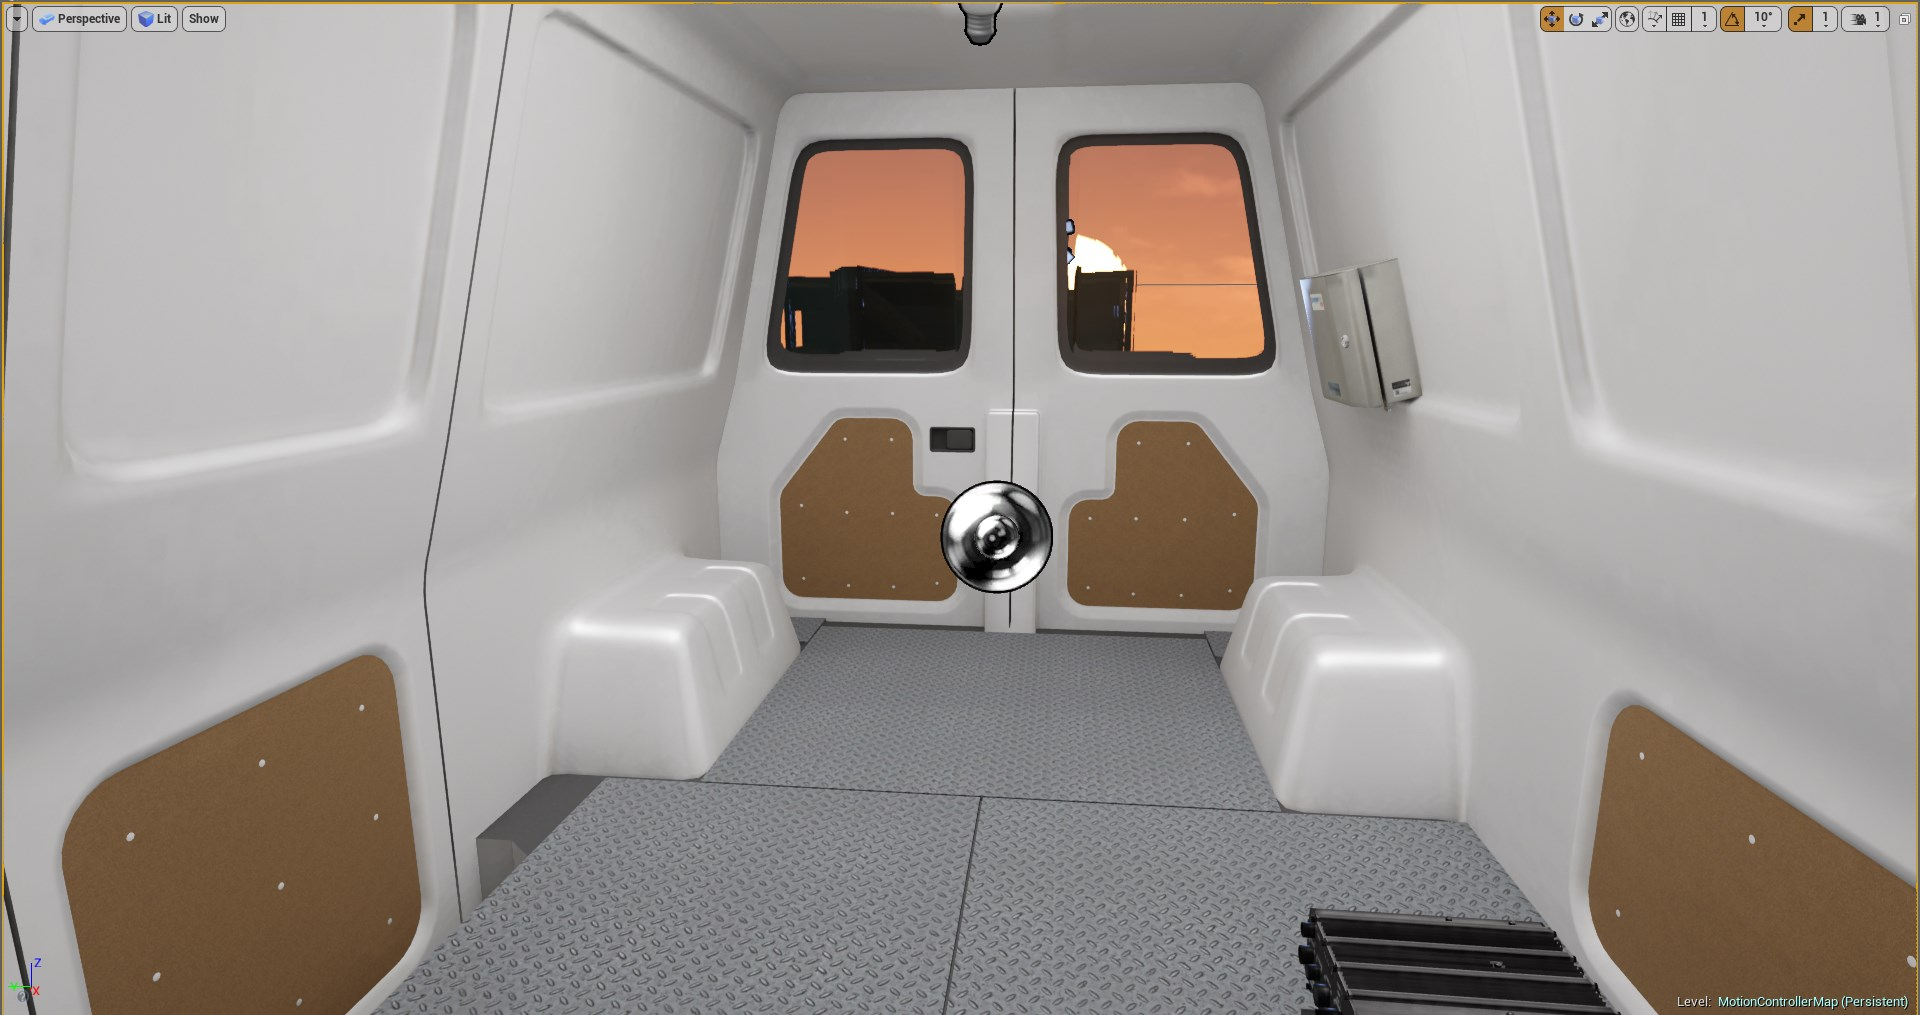
\includegraphics[width=\textwidth]{vehicle-interior}
	\caption{Starting Level Vehicle Interior}
	\label{fig:vehicle-interior}
\end{figure}
\par
Light sources are required to make meshes in the scene visible to the user. Two primary light sources are used in this level.\todo{Need to check from UE project}
\par
Layout of the hardware. \todo{Has to be decided when finalized}
\section{Glove calibration and tracking}
Hi5 VR Gloves require the user to go through a calibration process before use to ensure better finger tracking. This process needs to be done if the gloves have been turned on or a new person is going to be using the gloves. Noitom, the creators of the gloves, provide a sample UE4 project that includes the calibration process with instructions for the gloves. The calibration can be done with the stand-alone sample project, but to keep the final project self-contained the calibration will be added to the application.
\par
Inspecting the assets of the sample project reveals that two main actors are responsible for the instructions and calibration of the gloves. The UE4 editor comes with an asset migration tool which is used in this case to migrate these actors to the ObSAS VR project.
\section{Interacting with the virtual environment}
\section{Creating a context for training}

\par
\chapter{\MakeUppercase{Analyzing the mixed reality training application}}

\section{Future possibilities for development and improvement}


\newpage

\nocite{*}
\AtBeginEnvironment{thebibliography}{\linespread{1}\selectfont}
\bibliography{references}

\end{document}
